\section{附录：增强图与补充结果}
\subsection{附录增强图说明}
为增强正文分析的稳健性，本文补充图15至图21共7张附录增强图，涵盖模型残差诊断、增速脱钩、变量联动及情景分解等维度。附录图遵循``模型检验—结构观察—情景分解''逻辑组织，作为稳健性补强，不改变正文核心结论。

\begin{figure}[H]
    \centering
    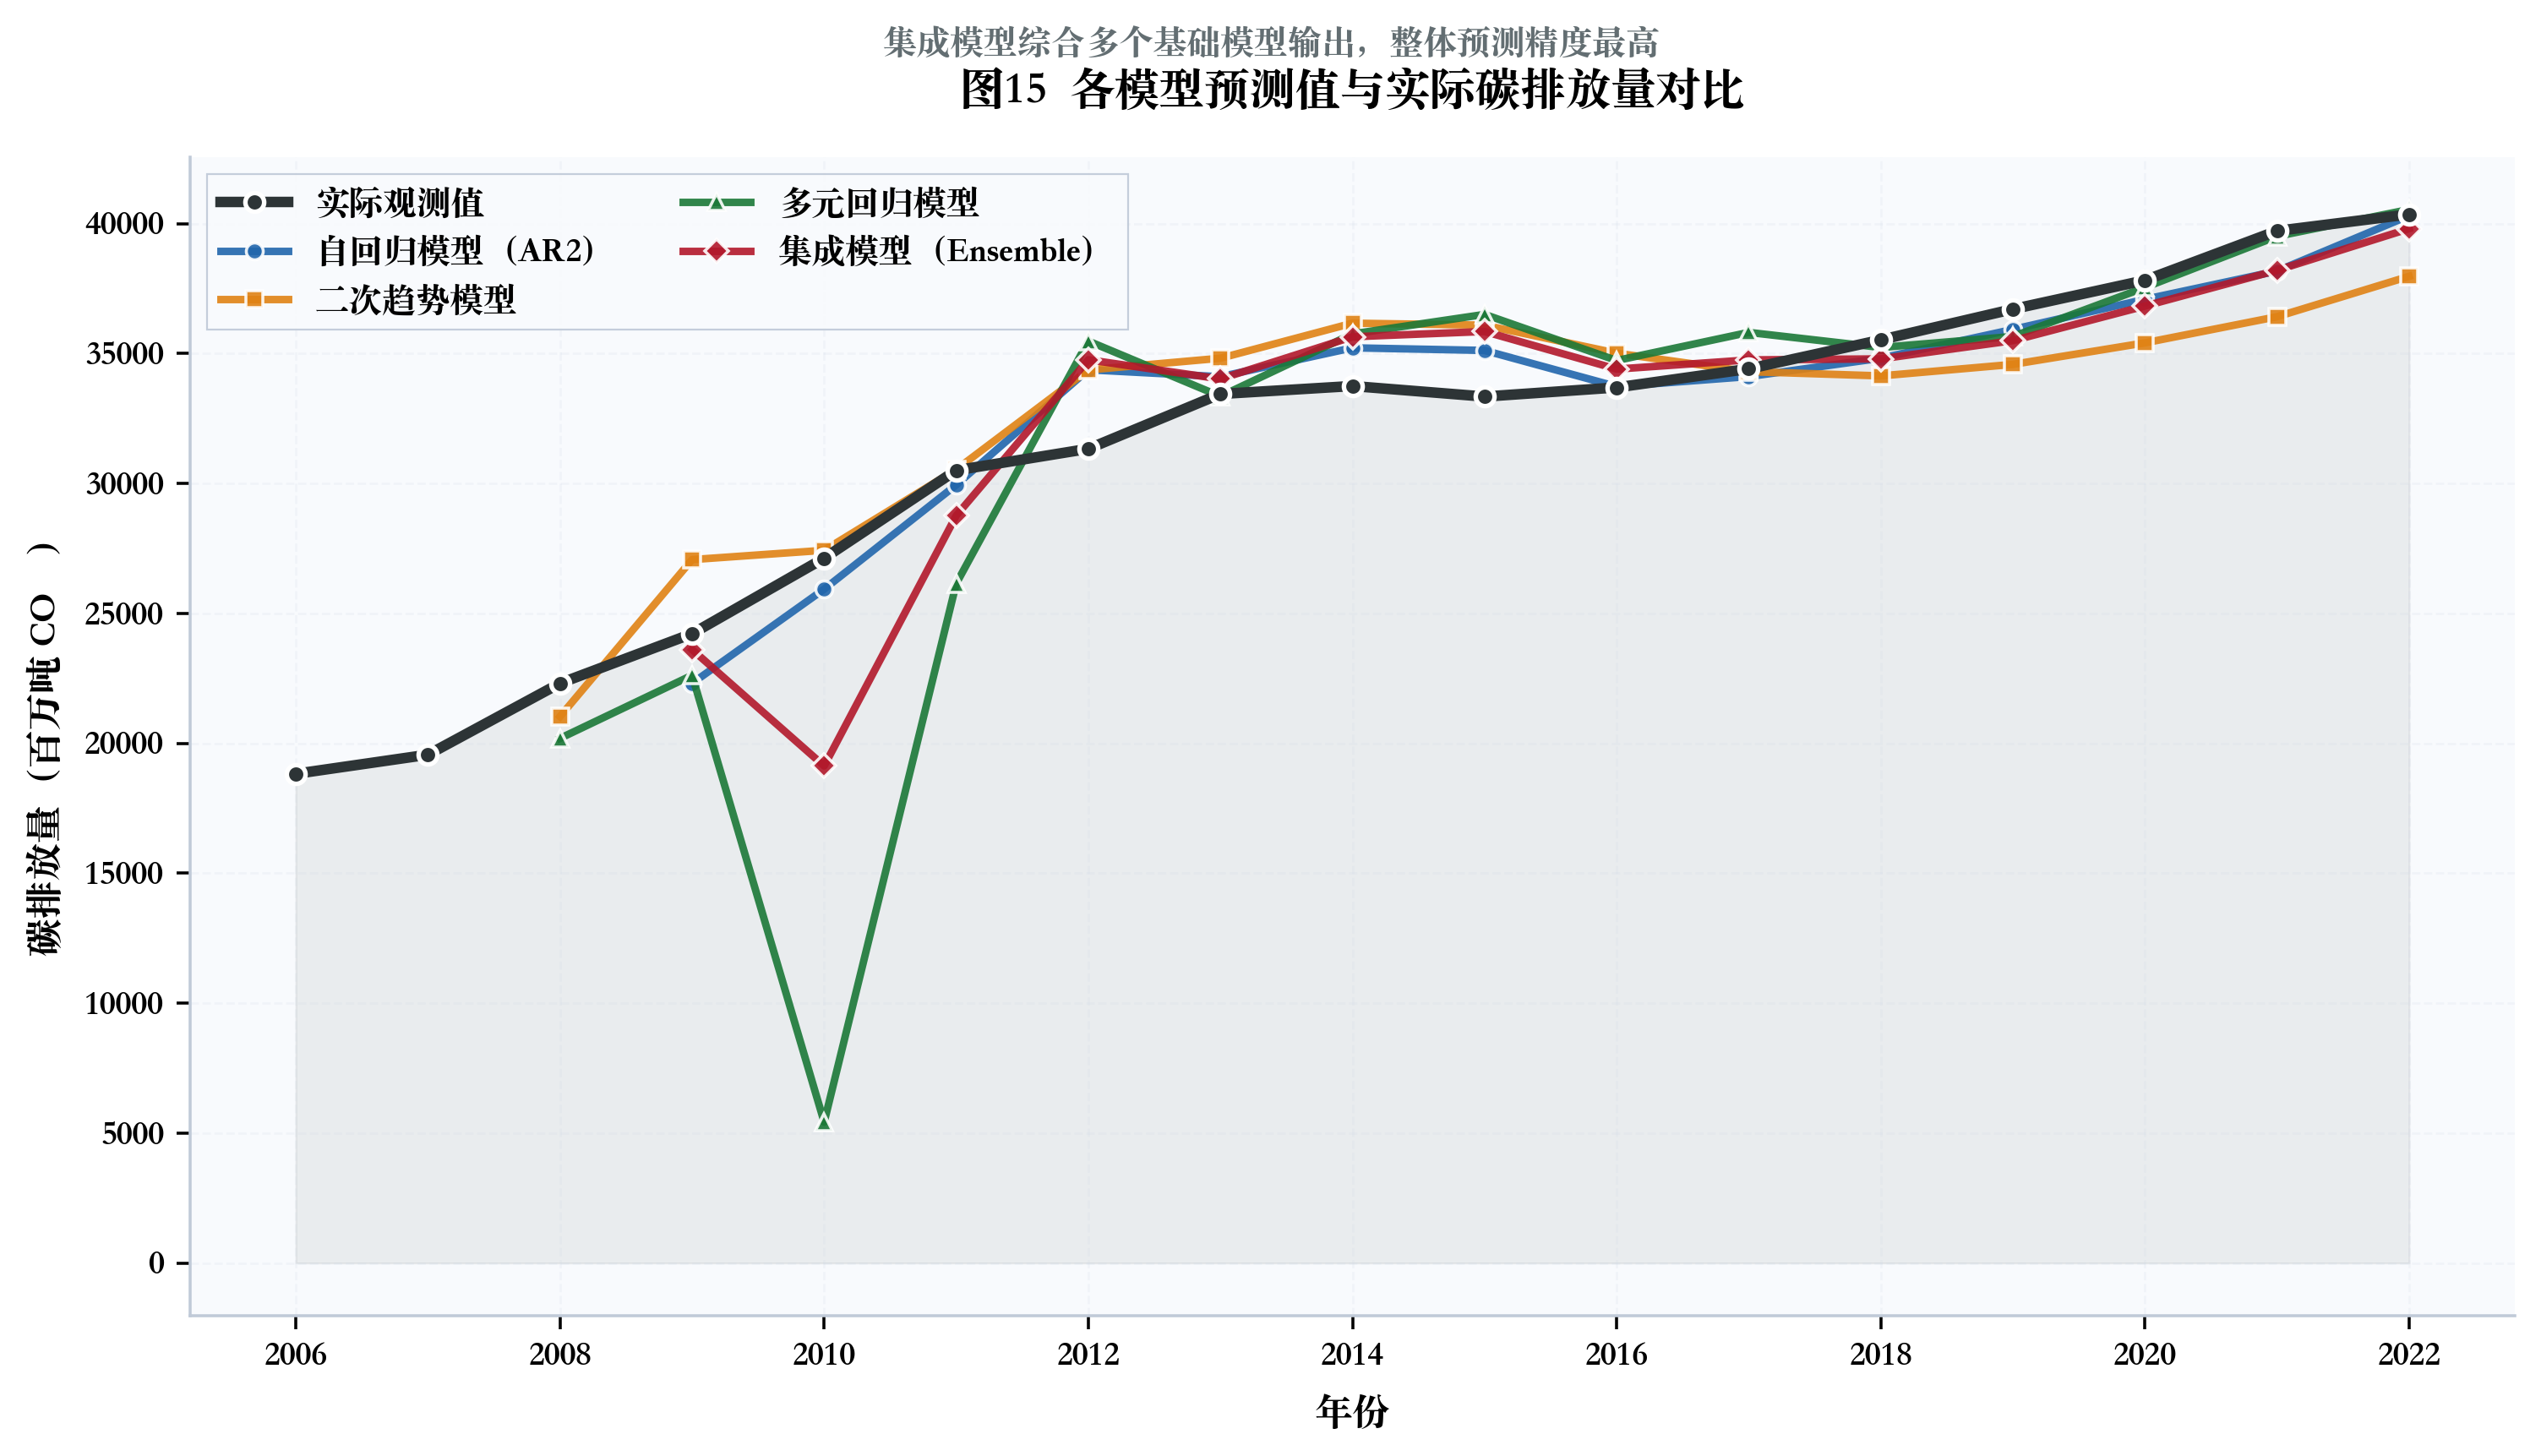
\includegraphics[width=0.82\textwidth]{../outputs/figures/Fig15_actual_vs_predicted.png}
    \caption{实际值与预测值对比图}
\end{figure}



\begin{figure}[H]
    \centering
    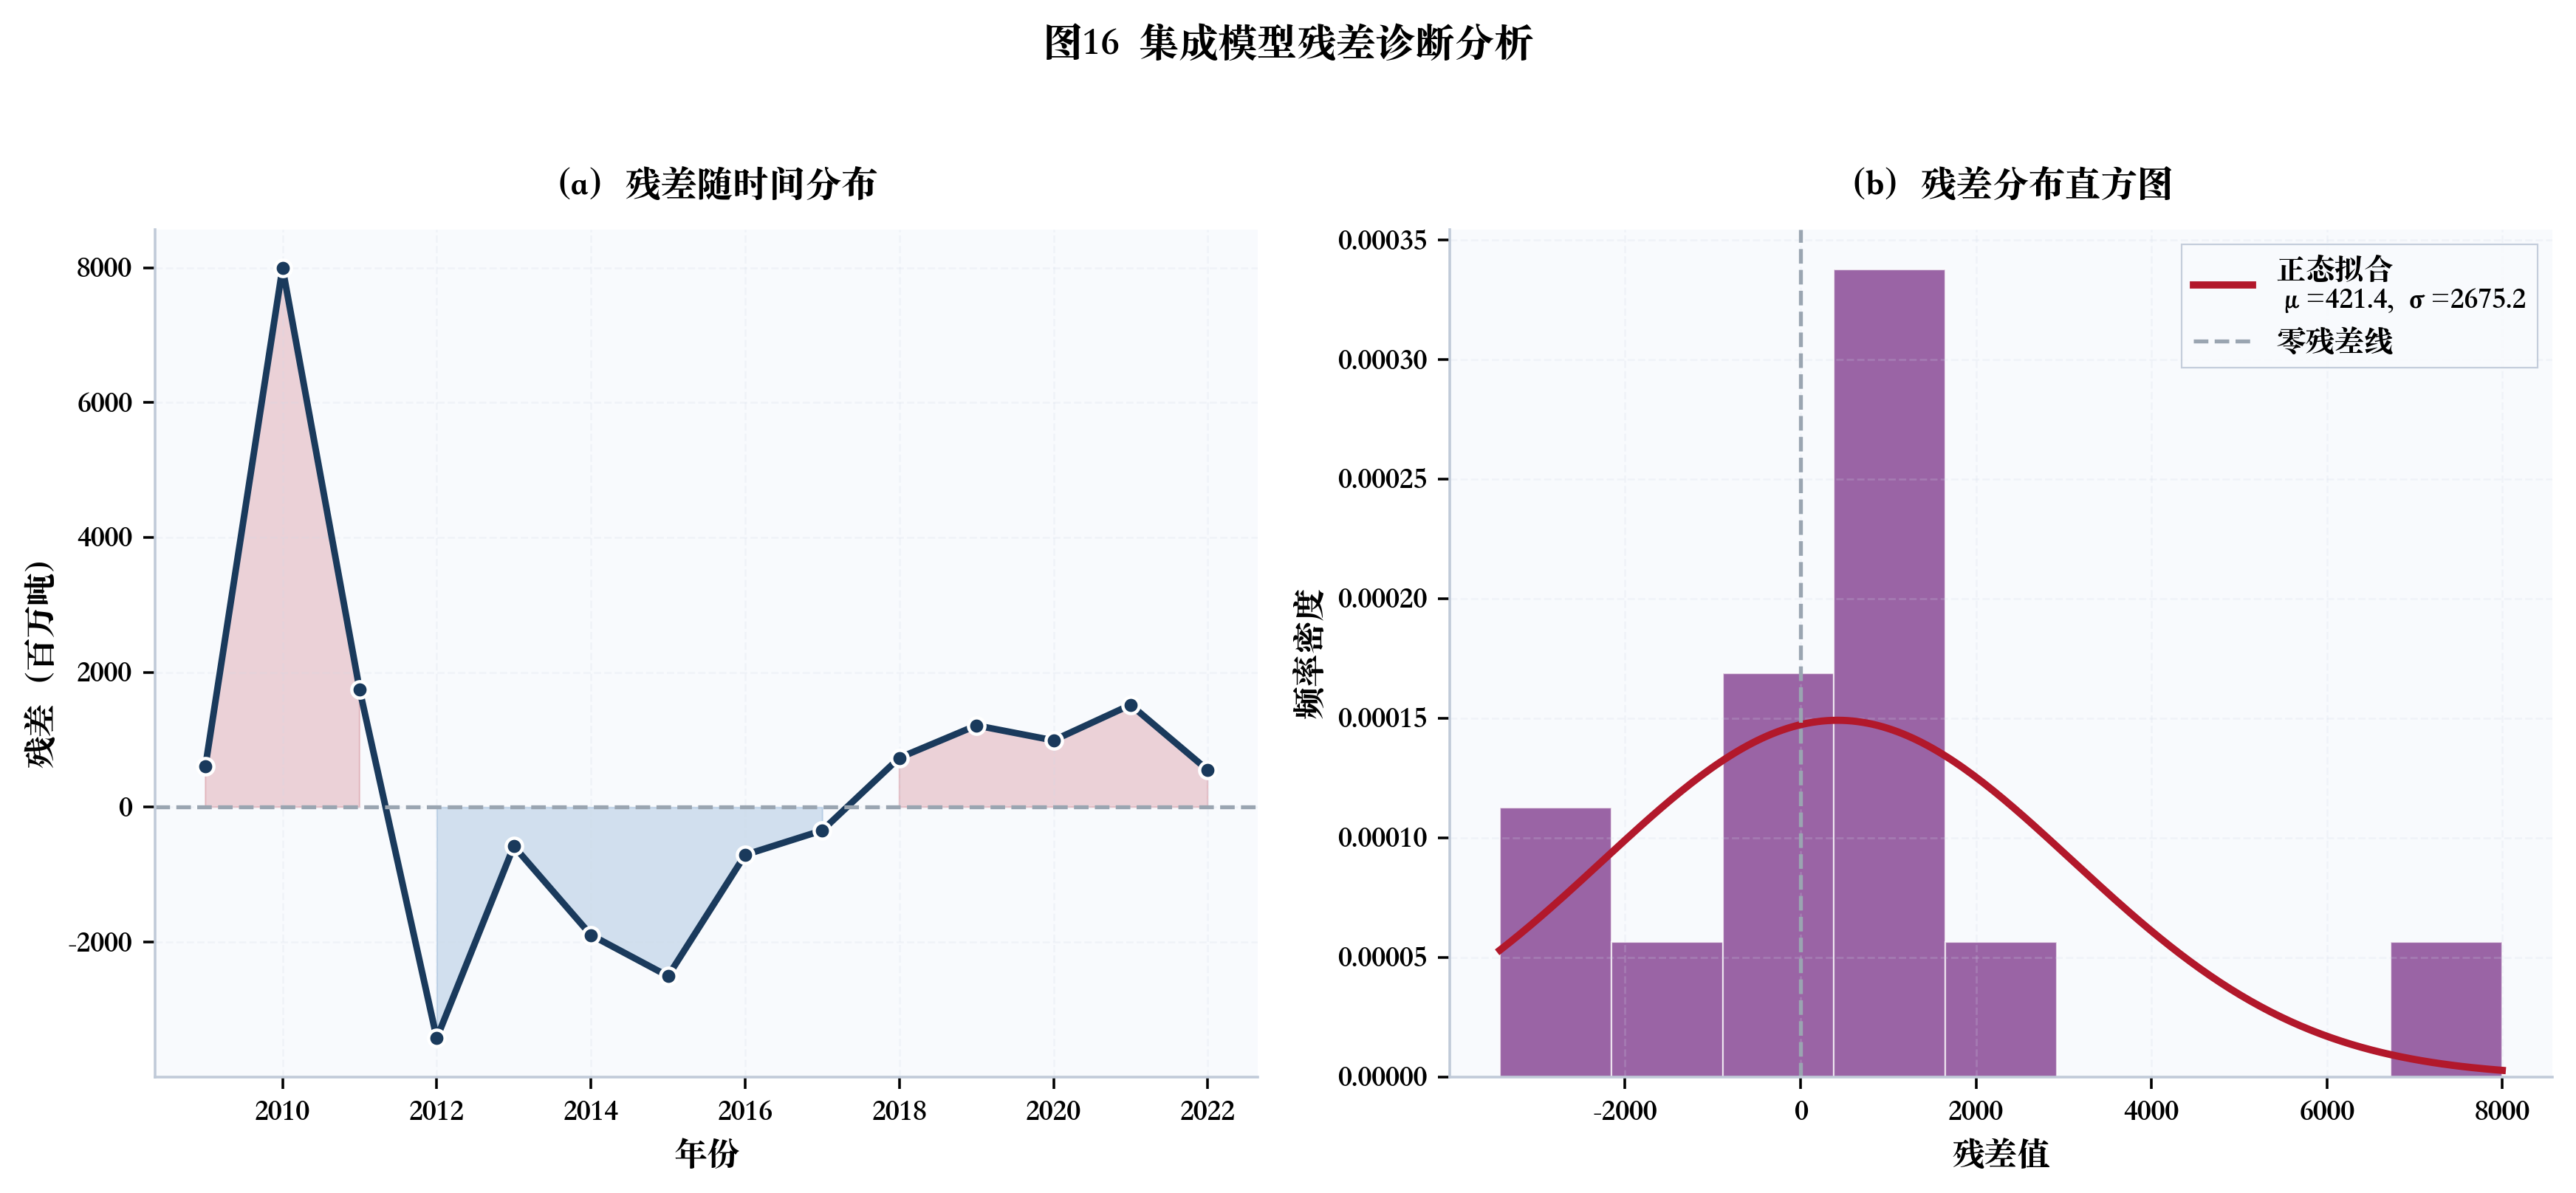
\includegraphics[width=0.92\textwidth]{../outputs/figures/Fig16_residual_diagnostics.png}
    \caption{集成模型残差诊断图}
\end{figure}



\begin{figure}[H]
    \centering
    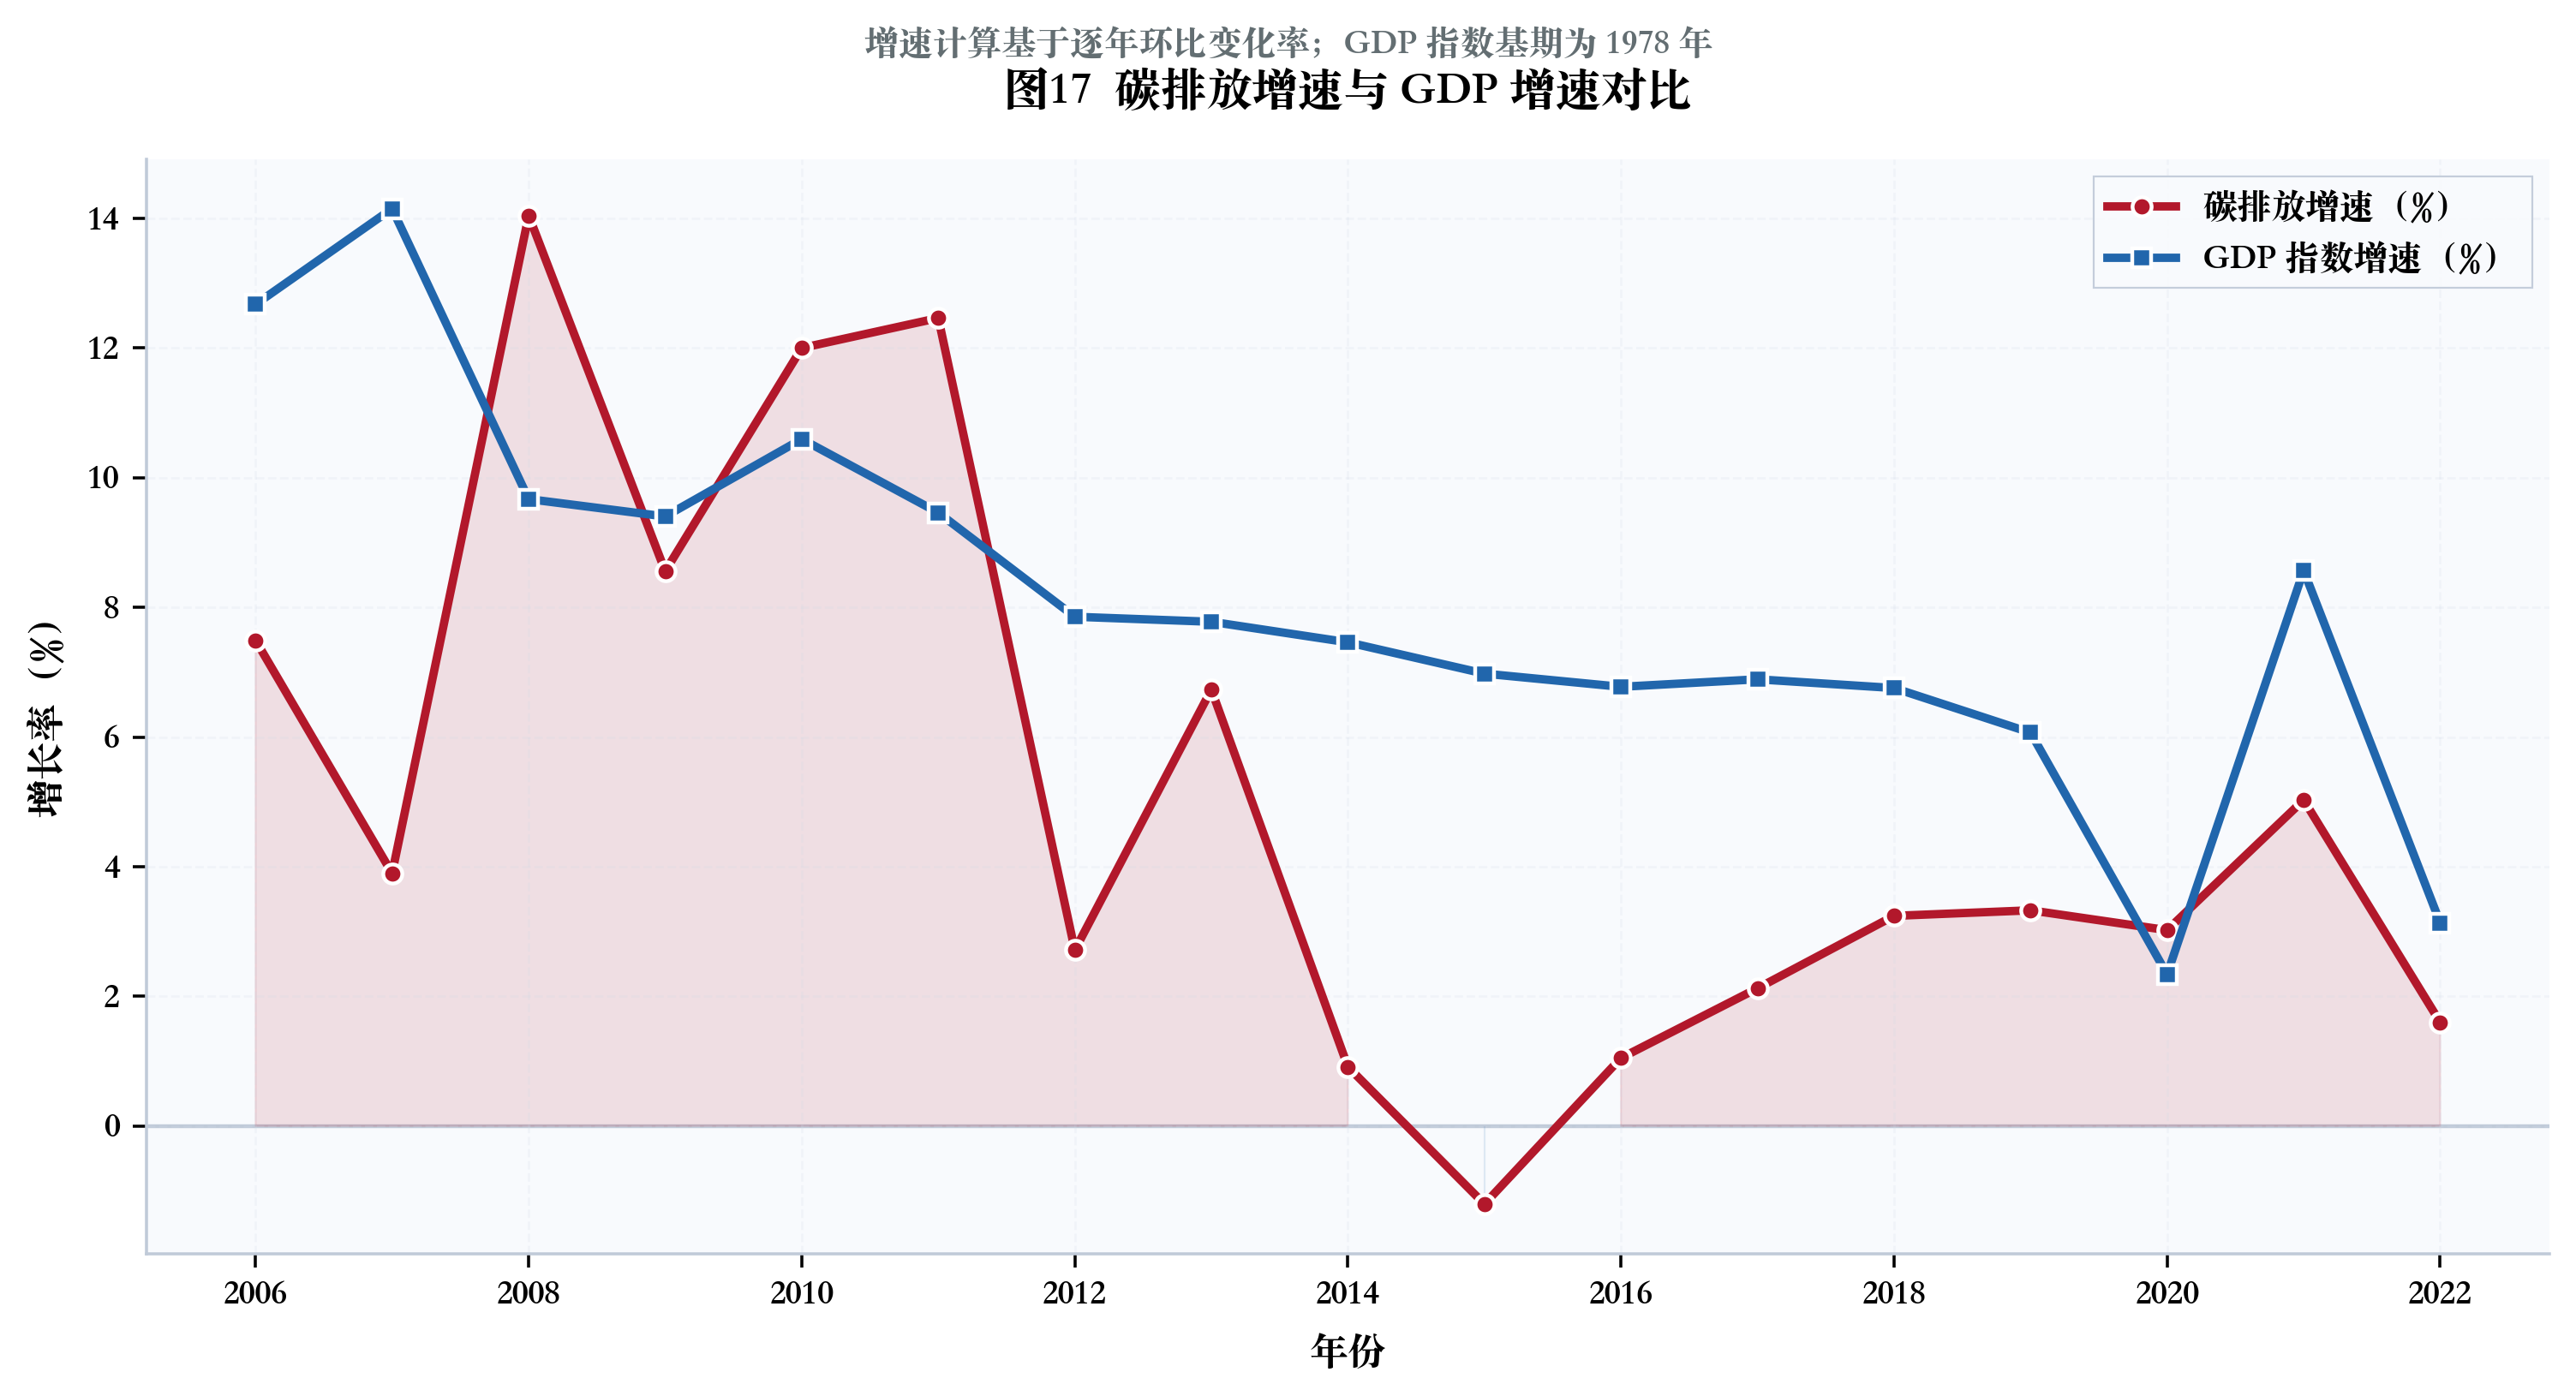
\includegraphics[width=0.82\textwidth]{../outputs/figures/Fig17_growth_rate_comparison.png}
    \caption{碳排放与GDP增速对比图}
\end{figure}



\begin{figure}[H]
    \centering
    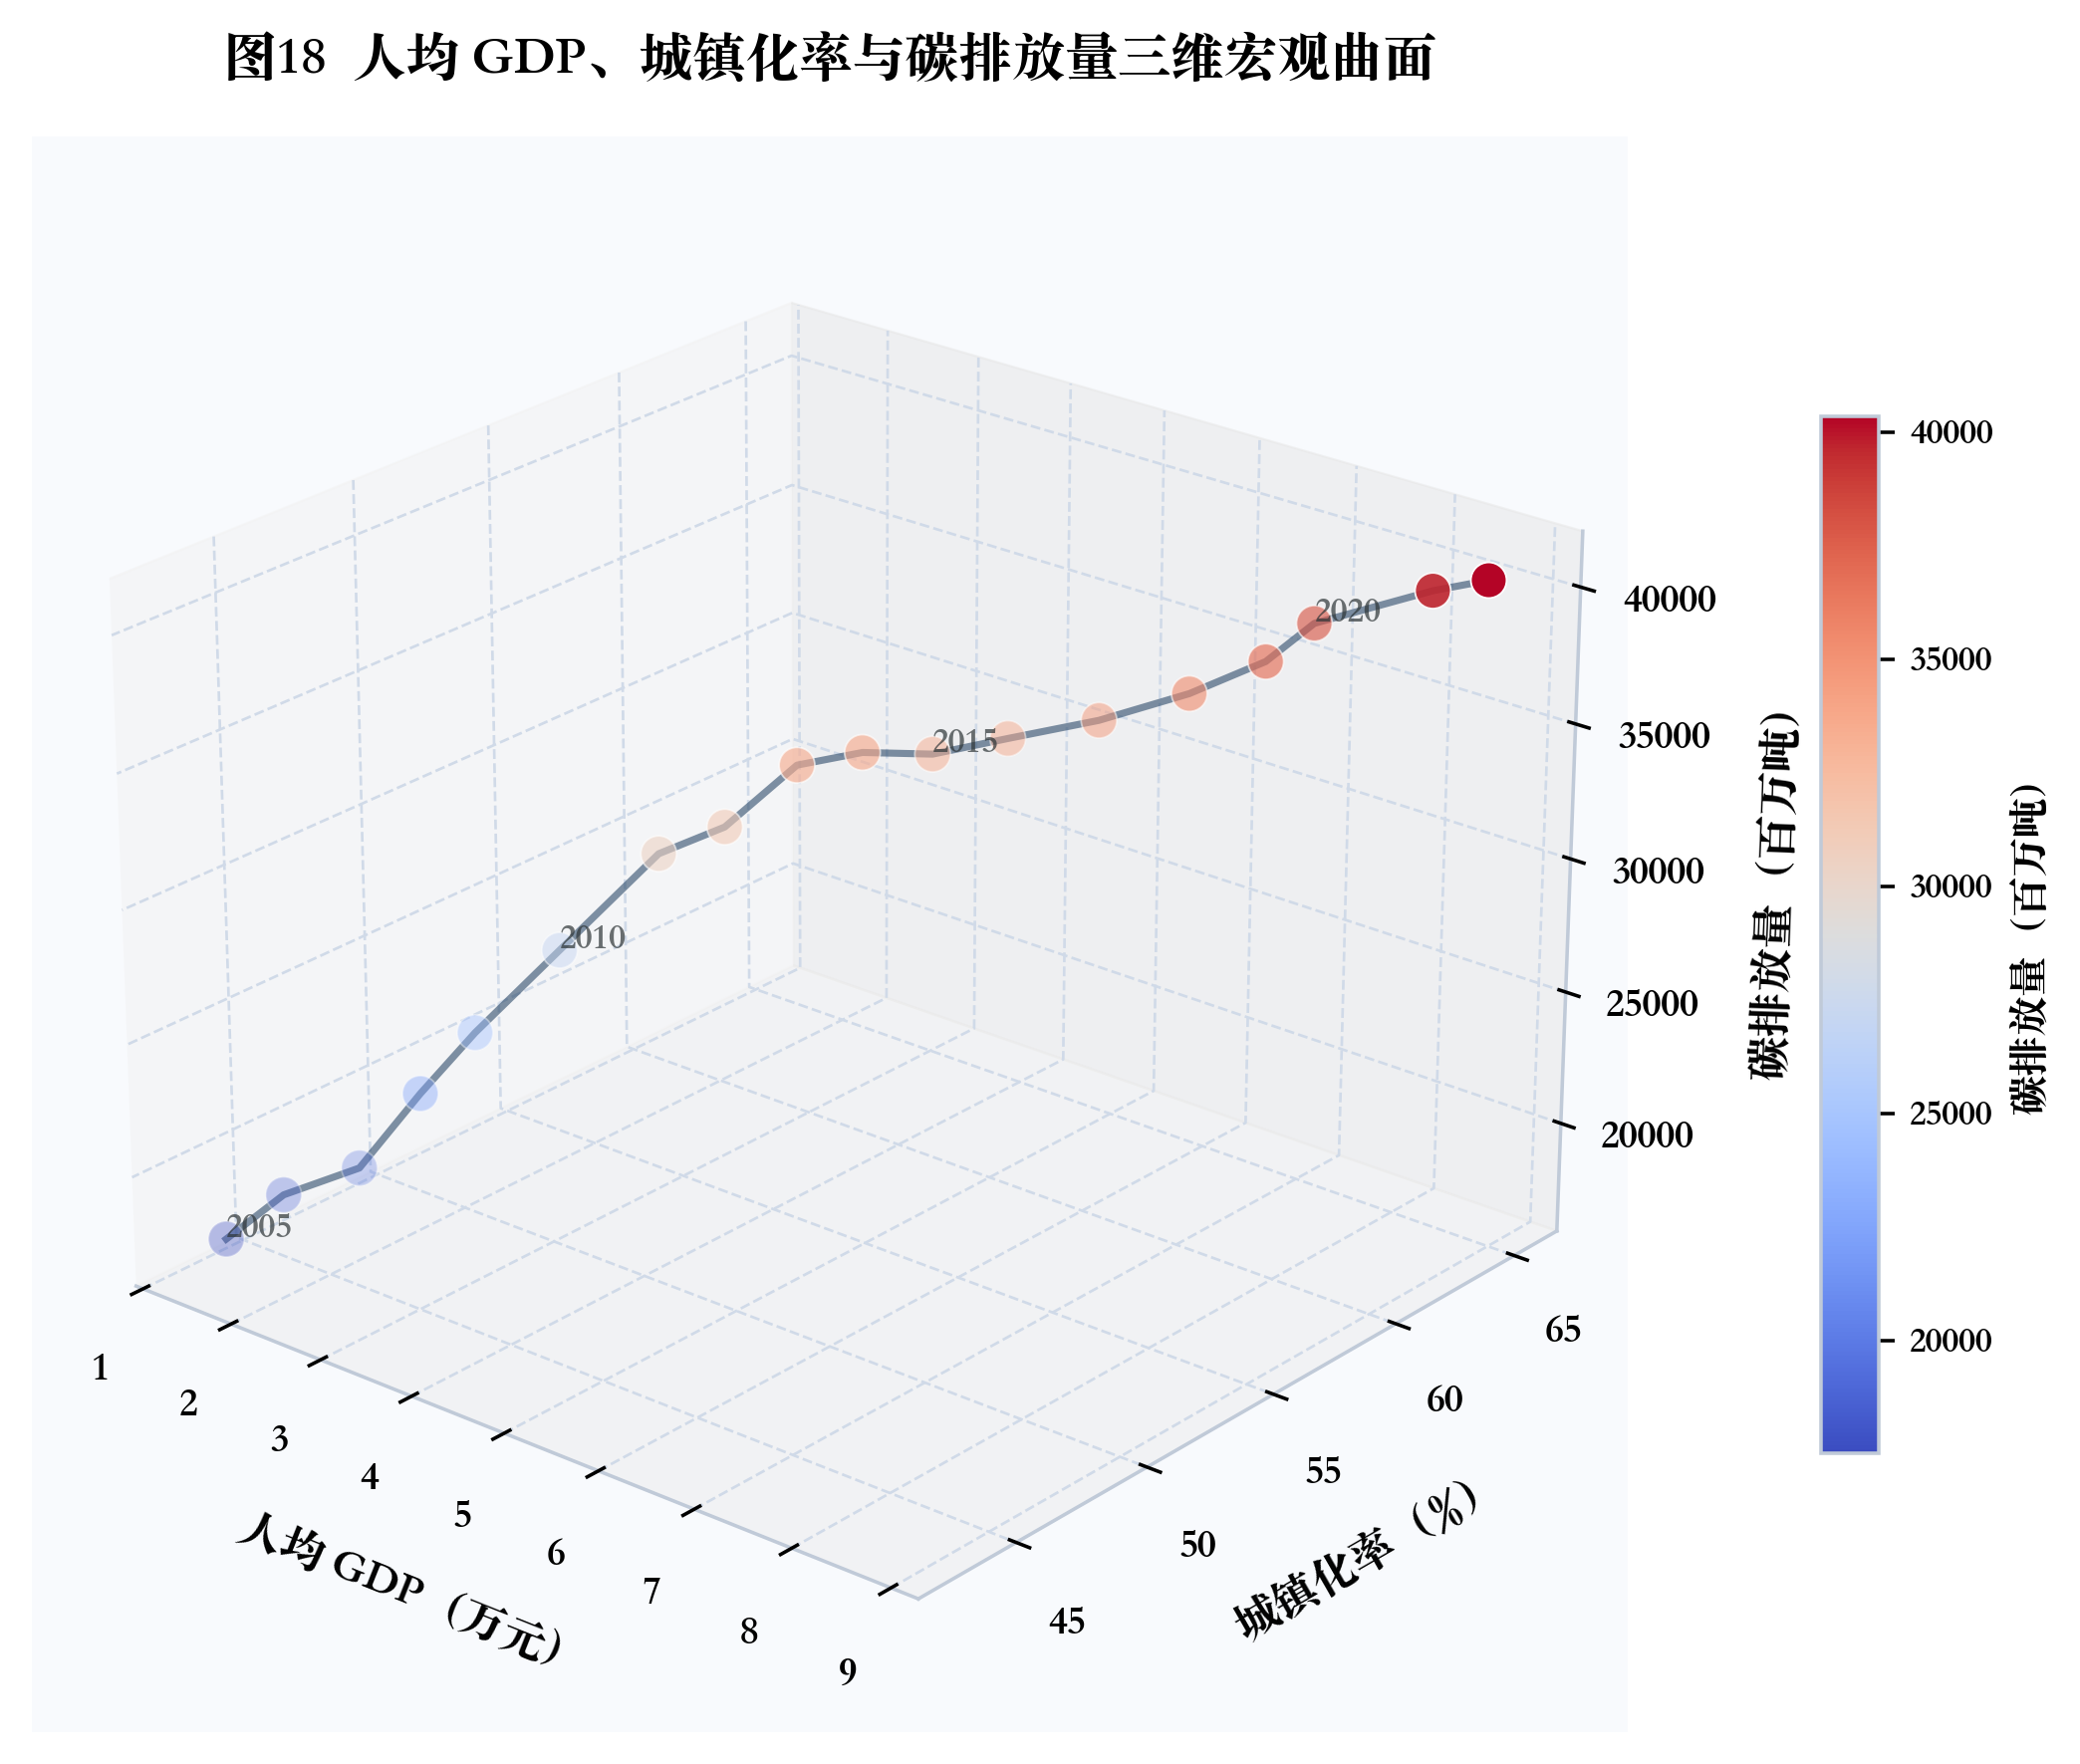
\includegraphics[width=0.78\textwidth]{../outputs/figures/Fig18_3d_macro_surface.png}
    \caption{GDP、城镇化与碳排放三维响应图}
\end{figure}



\begin{figure}[H]
    \centering
    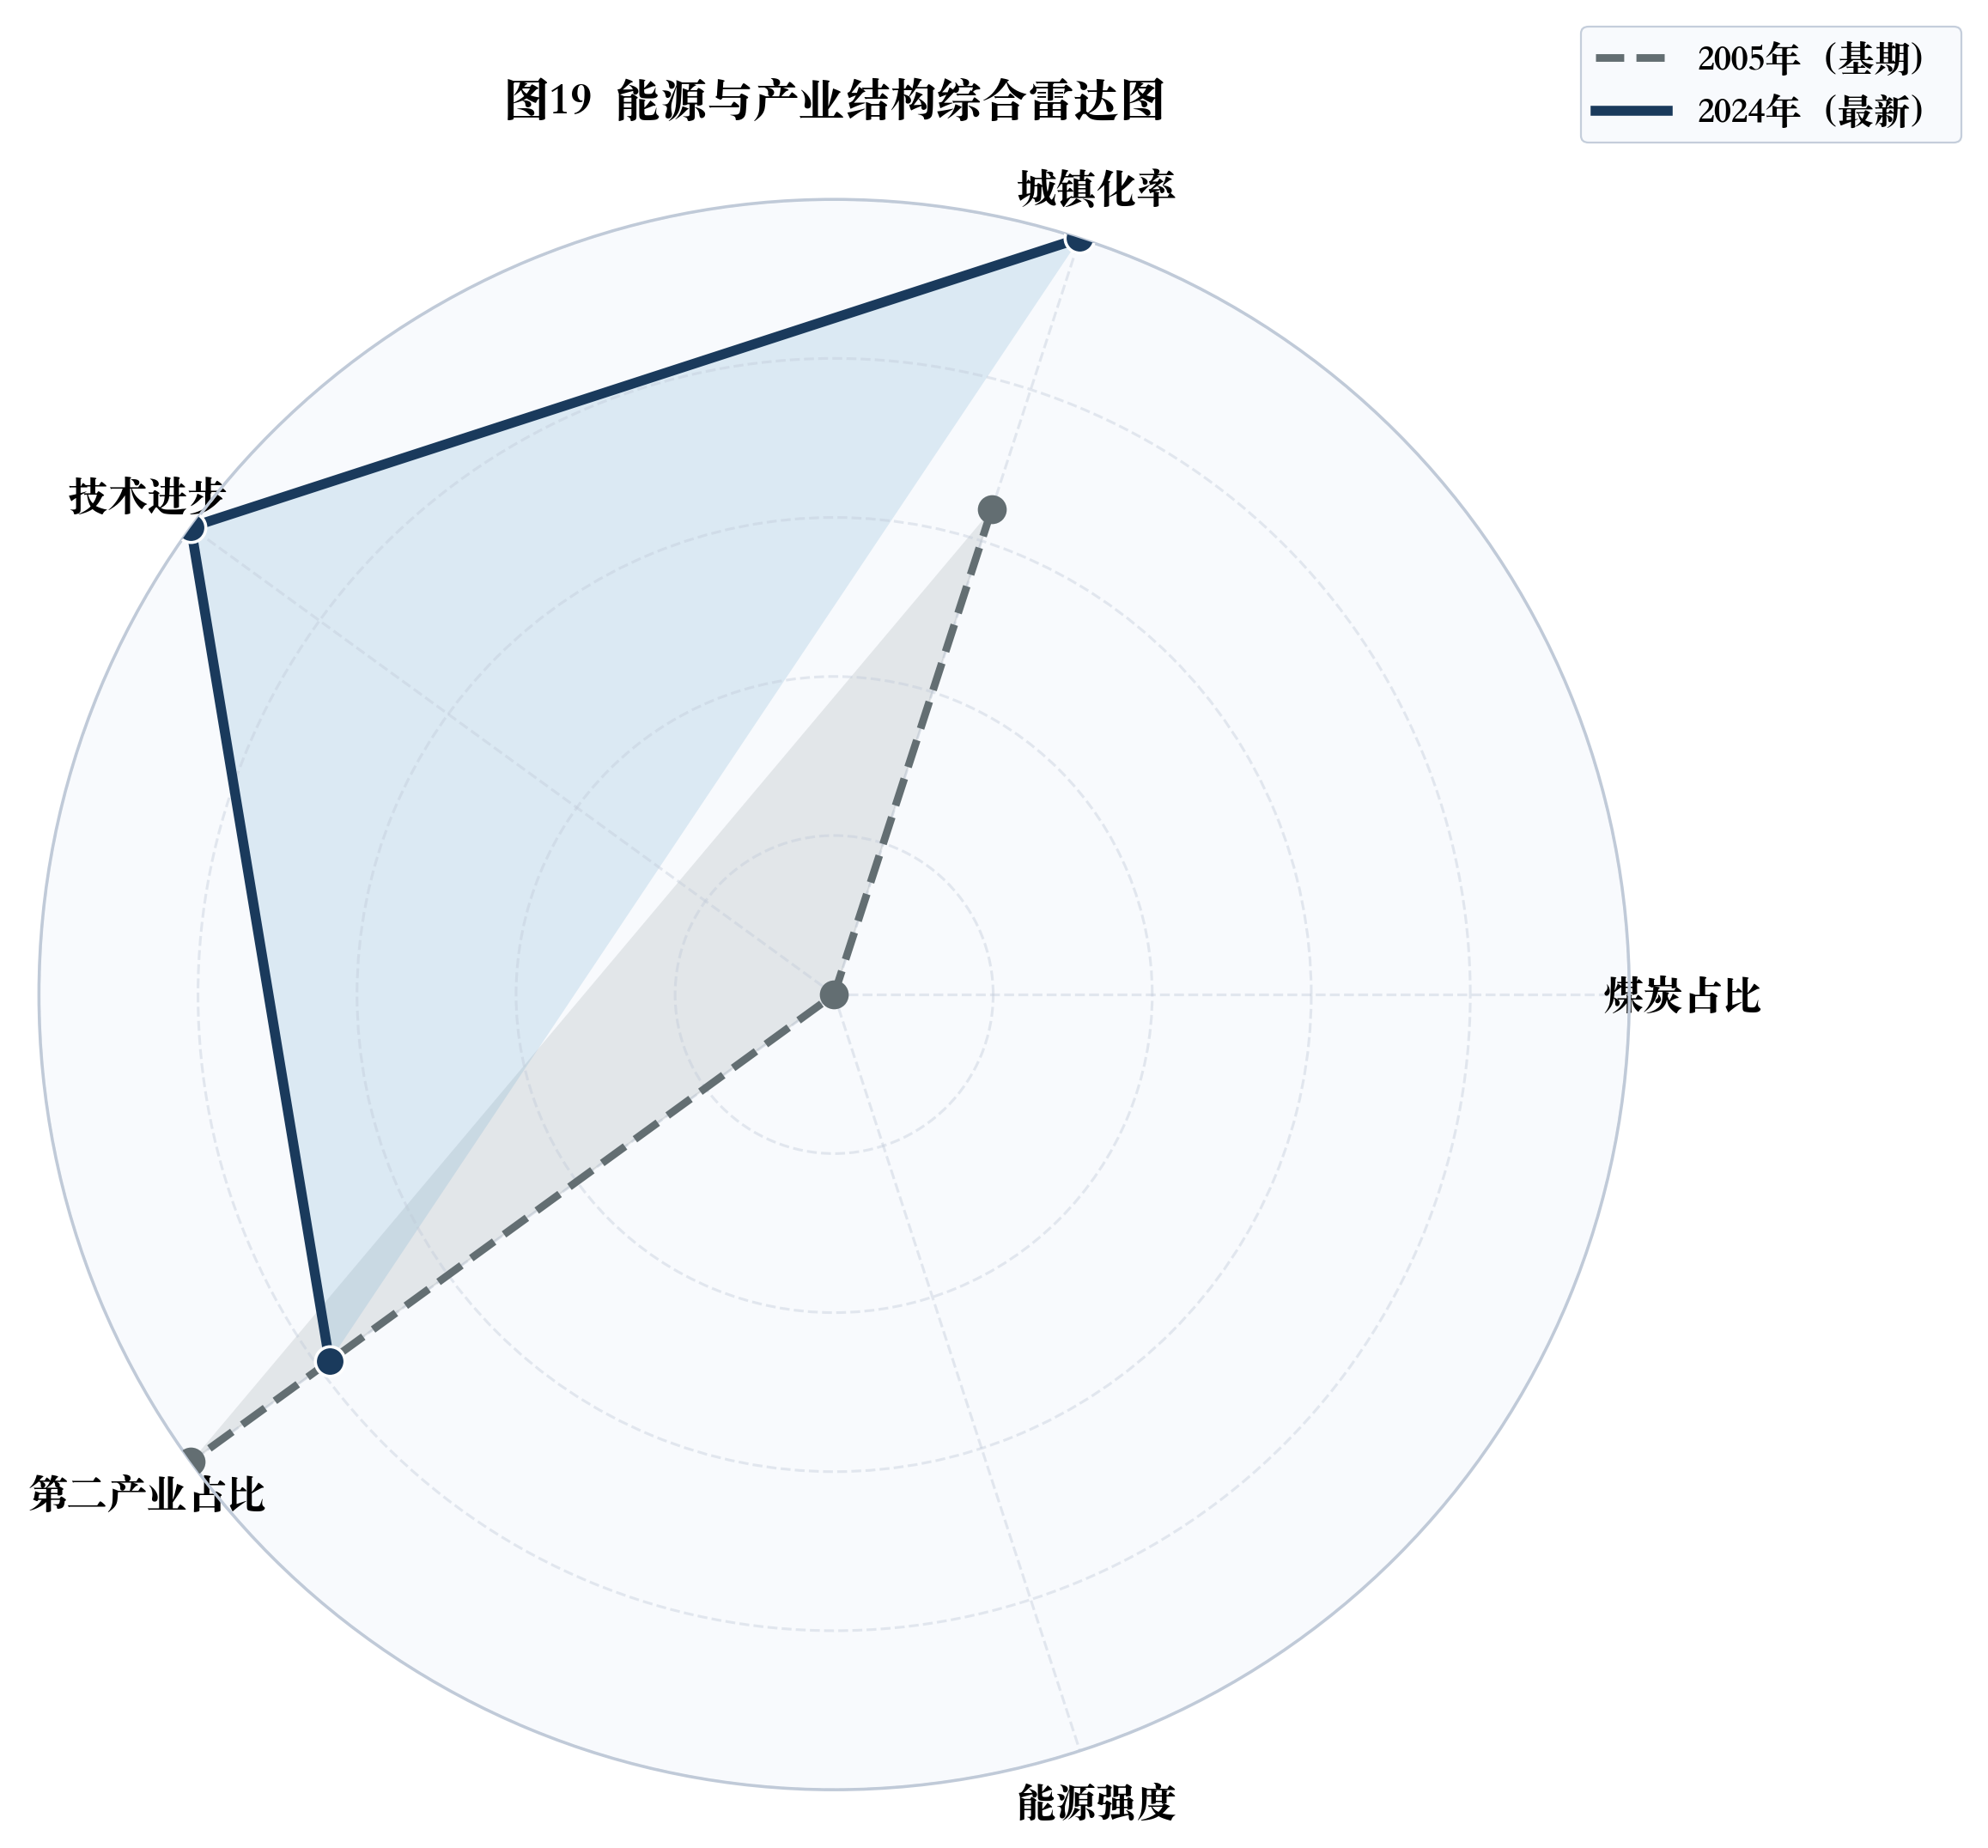
\includegraphics[width=0.62\textwidth]{../outputs/figures/Fig19_energy_radar.png}
    \caption{能源与结构特征雷达图}
\end{figure}



\begin{figure}[H]
    \centering
    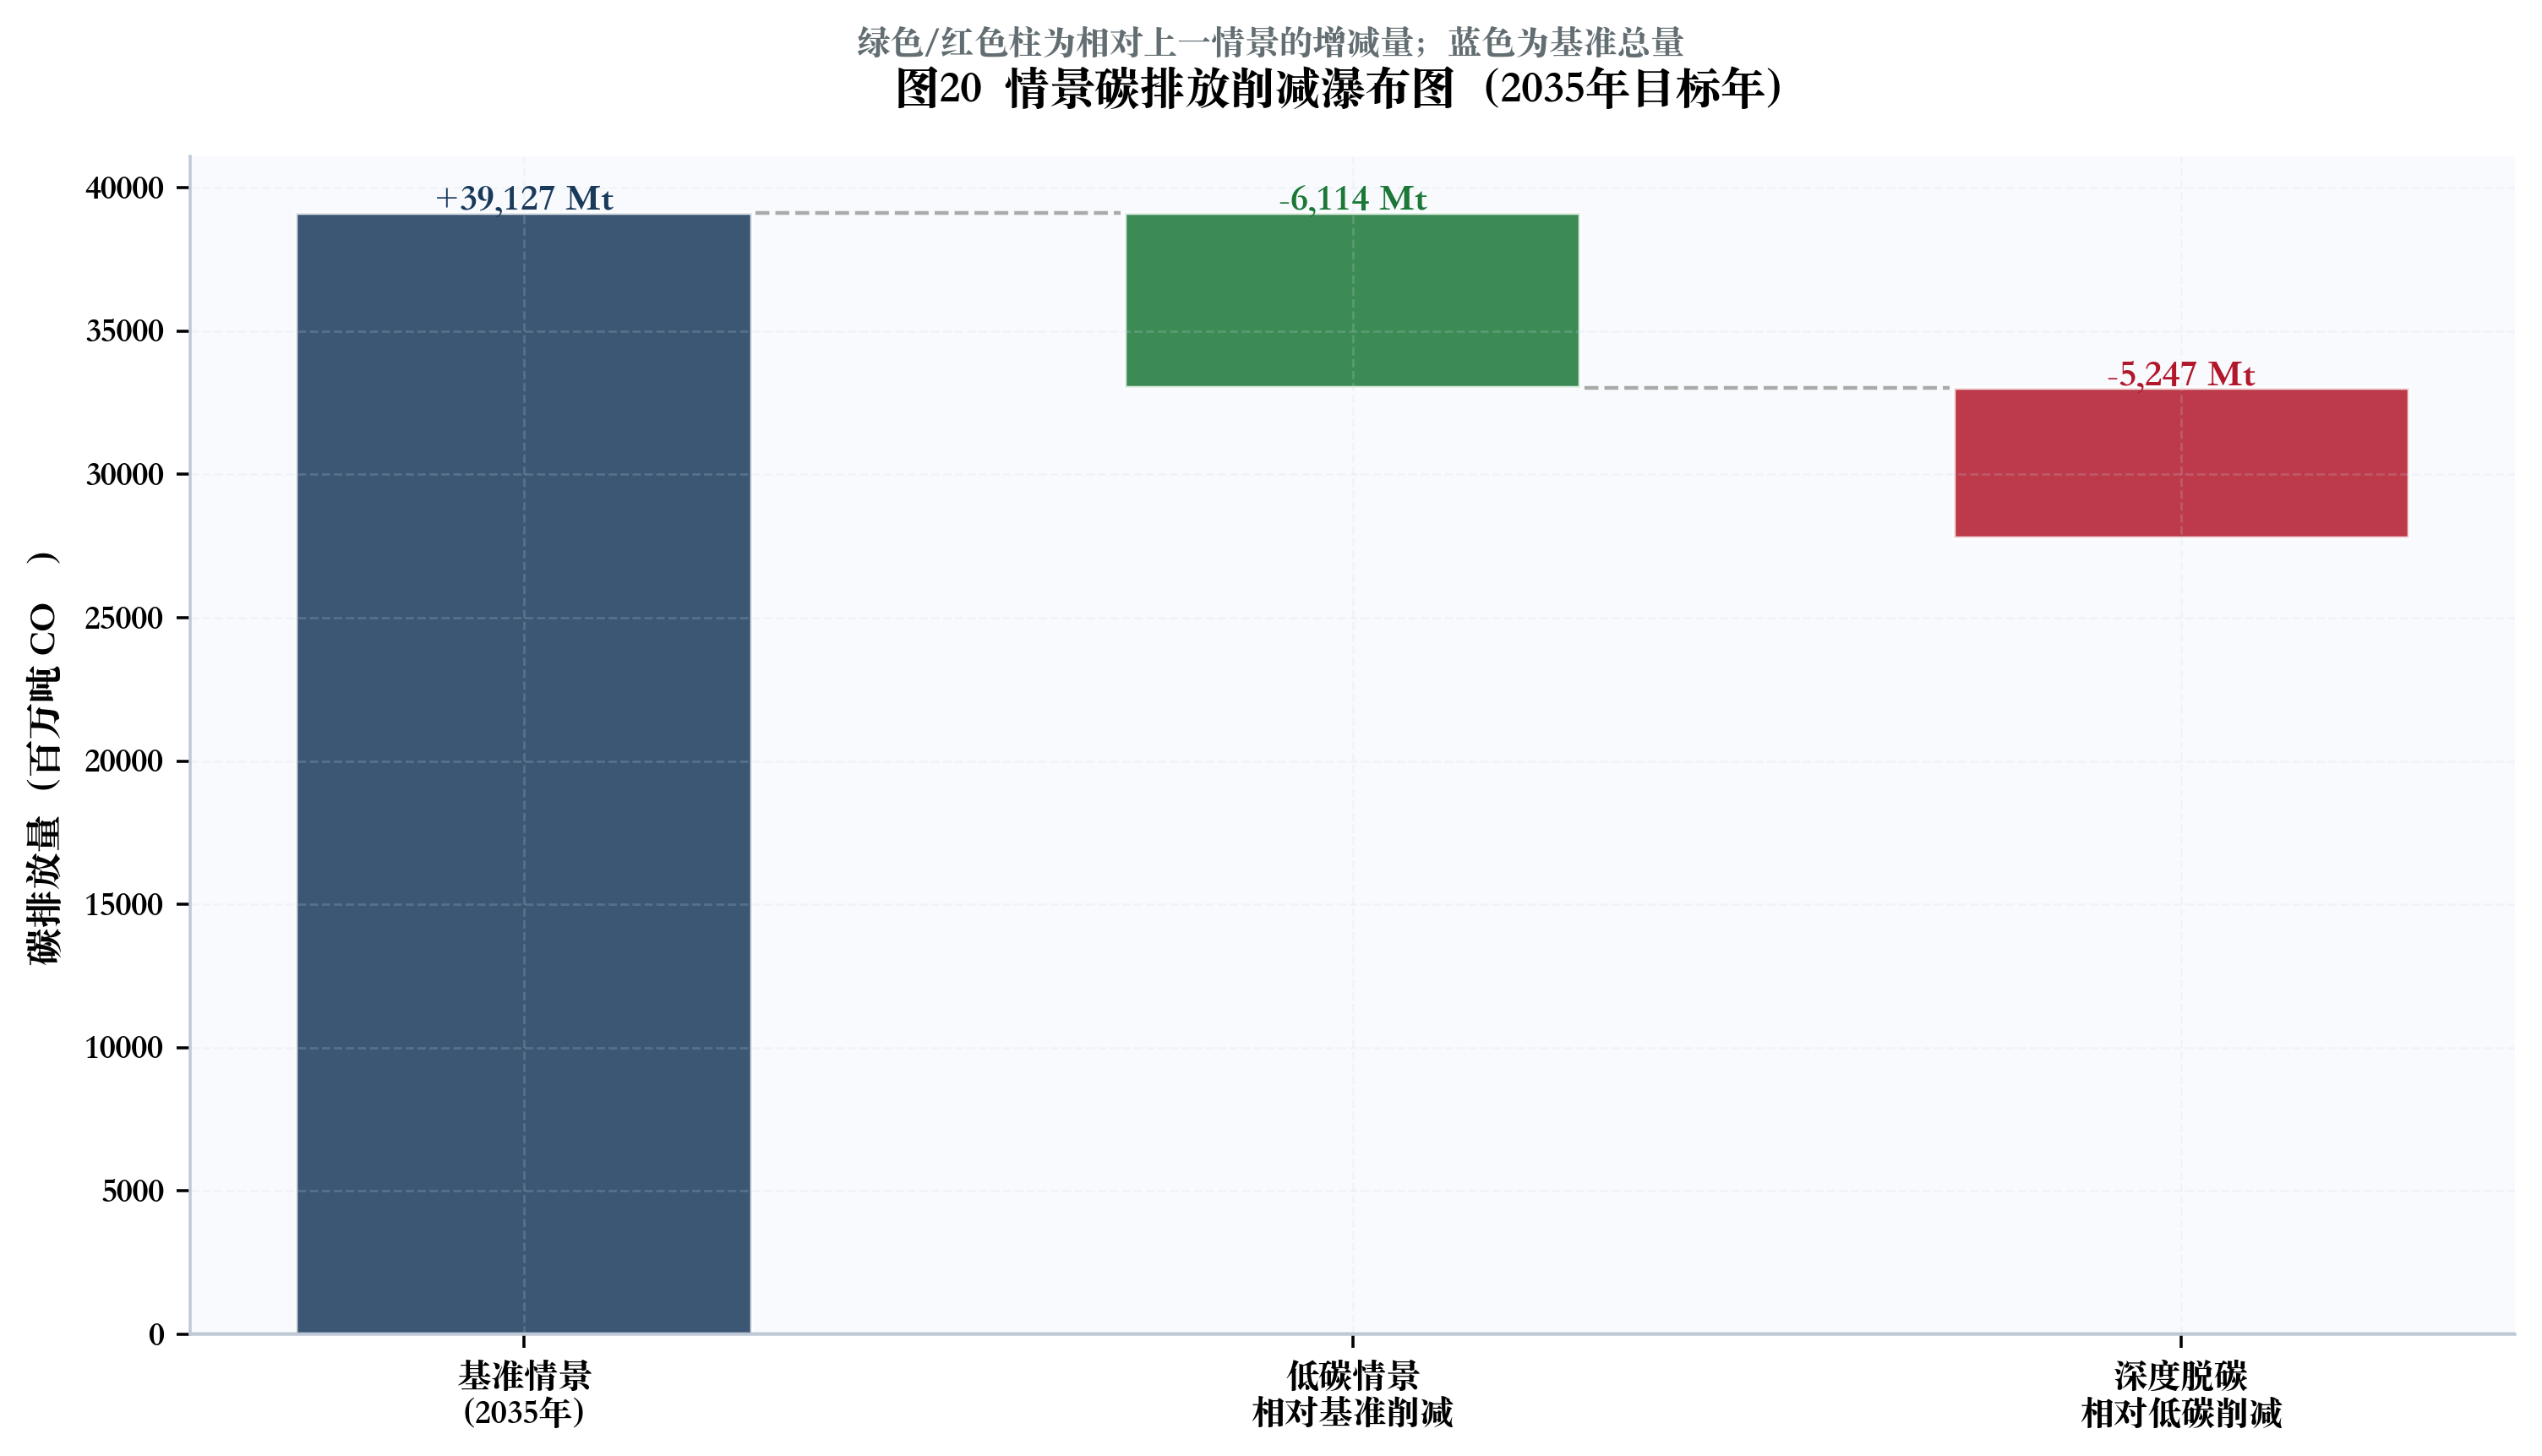
\includegraphics[width=0.82\textwidth]{../outputs/figures/Fig20_scenario_waterfall.png}
    \caption{2035年情景差异瀑布分解图}
\end{figure}



\begin{figure}[H]
    \centering
    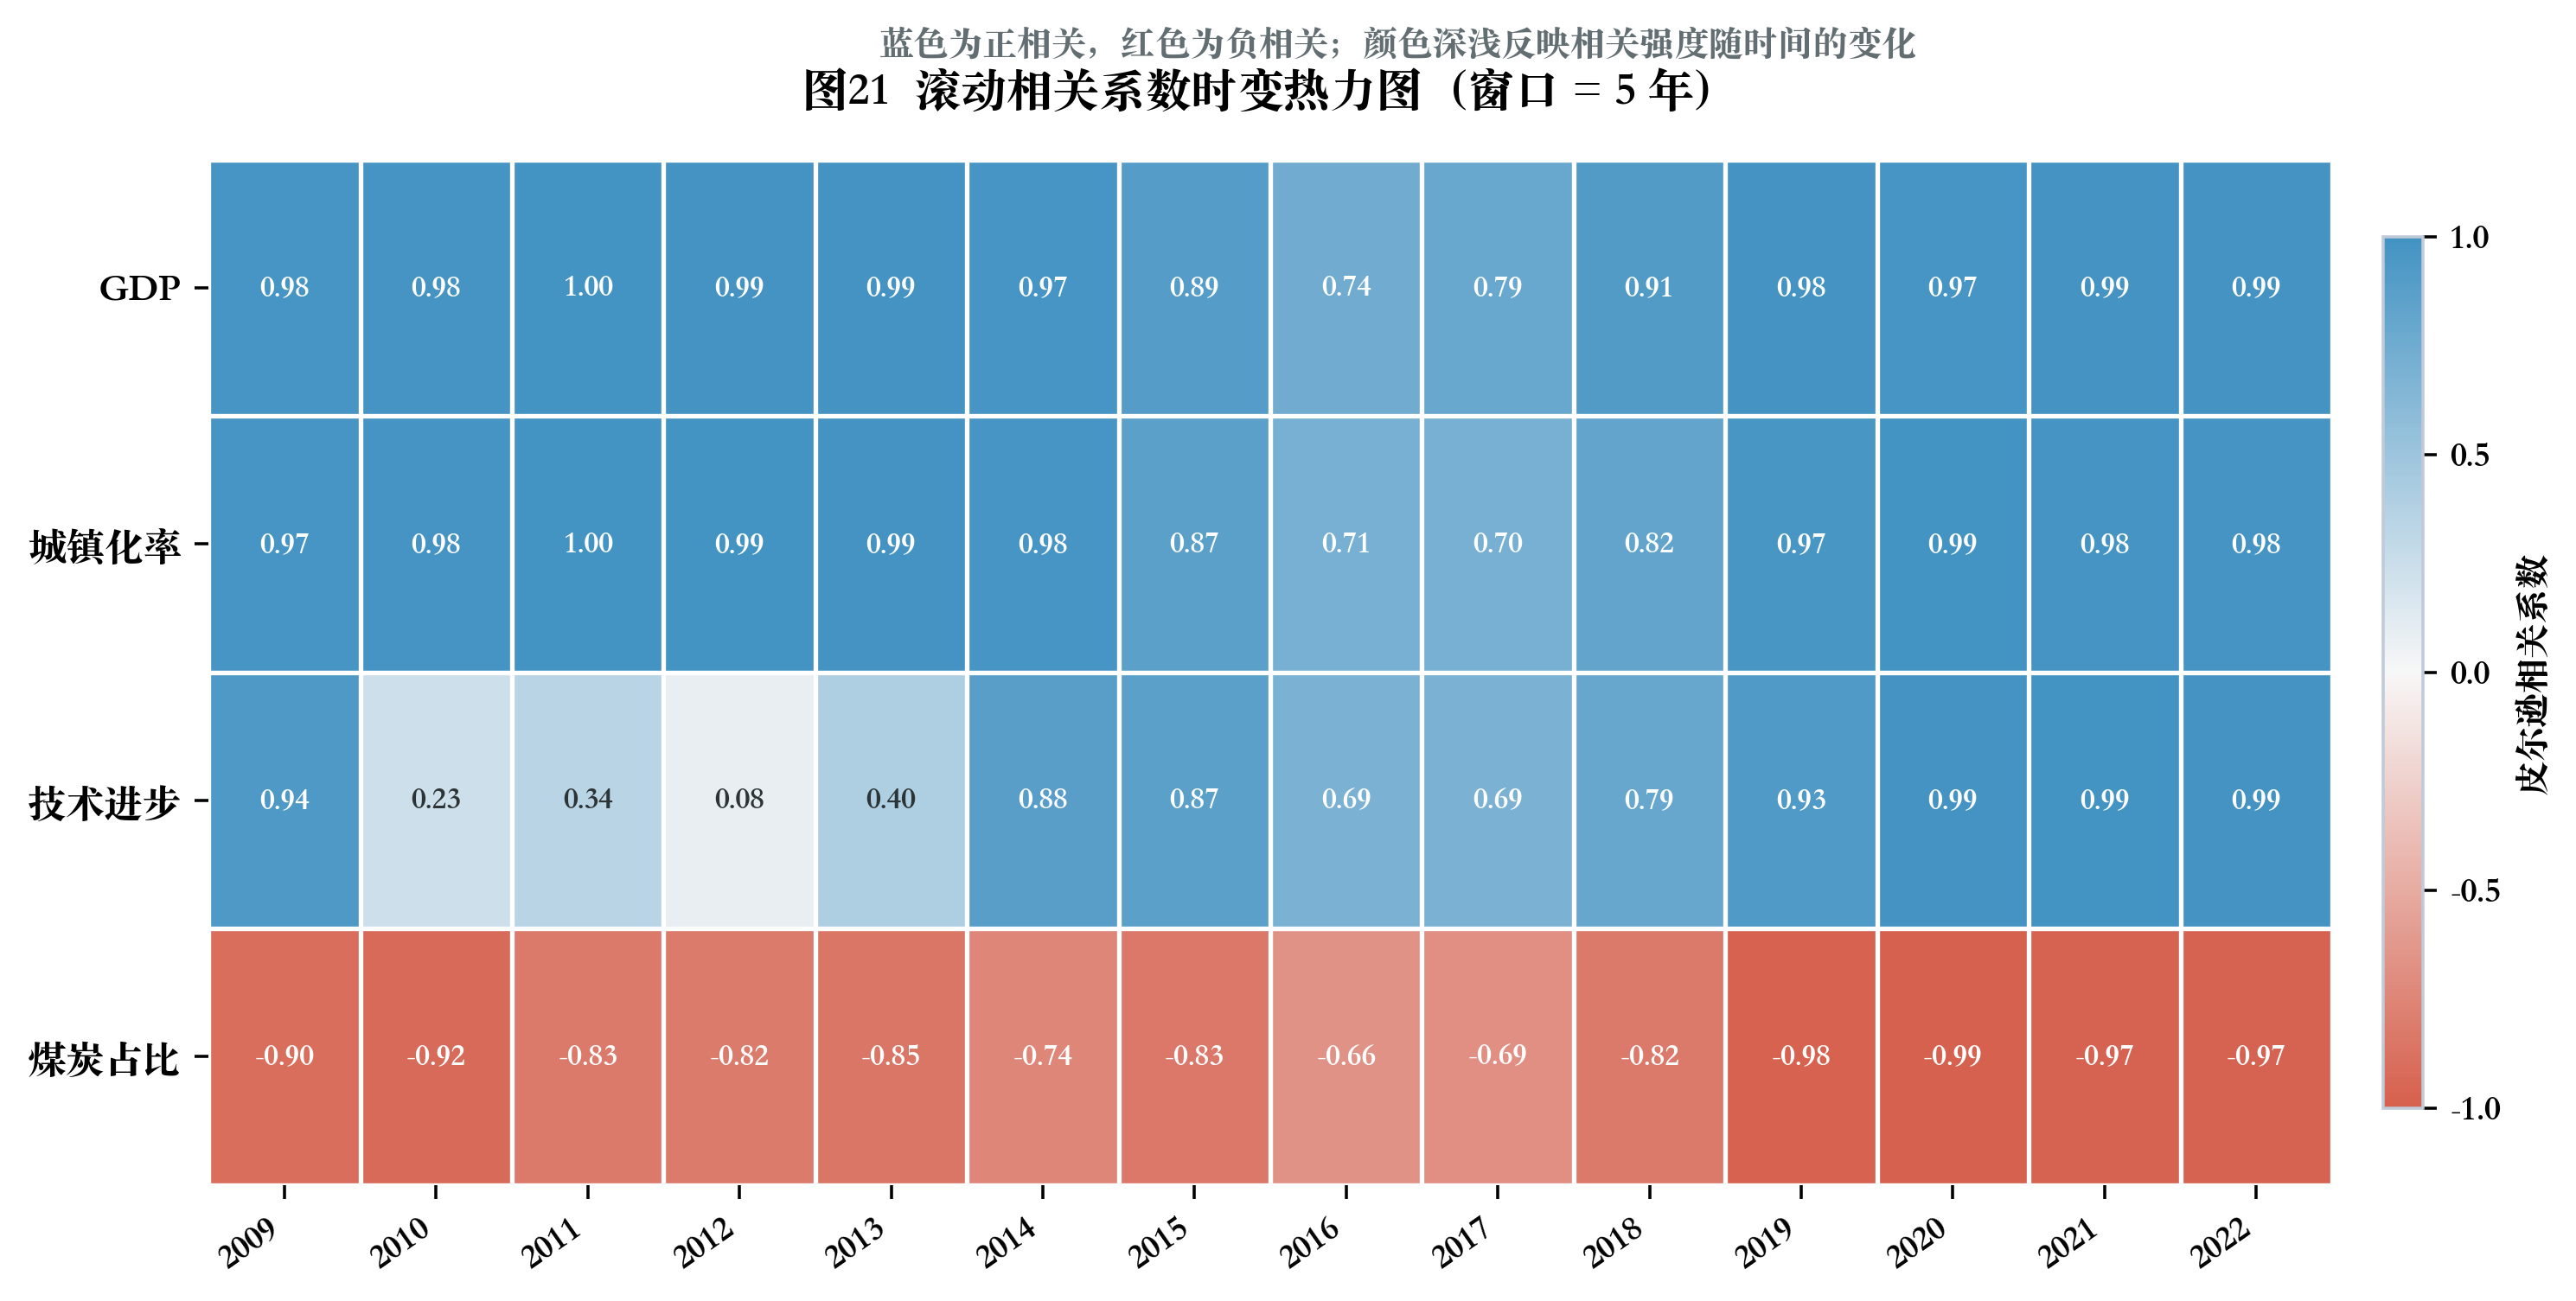
\includegraphics[width=0.88\textwidth]{../outputs/figures/Fig21_rolling_correlation_heatmap.png}
    \caption{滚动相关热力图}
\end{figure}



\subsection{附录表与补充解释}
附录表集中呈现样本描述性统计，明确变量量级与波动范围，为正文弹性系数解释与情景设定提供量纲支撑。综合附录图表，本文主结论在不同诊断视角下保持一致，附录结果视为对正文结论的稳健性补强。

\begin{table}[H]
\centering
\caption{样本描述性统计}
\begin{tabular}{ccccc}
\toprule
变量 & 均值 & 标准差 & 最小值 & 最大值 \\
\midrule
CO2 emissions & 30566.50 & 7257.68 & 17516.39 & 40358.26 \\
Population & 1368.14 & 37.21 & 1307.56 & 1412.60 \\
GDP & 654617.21 & 329391.17 & 189907.50 & 1234029.40 \\
GDP per capita & 4.73 & 2.28 & 1.45 & 8.74 \\
Urbanization & 0.55 & 0.07 & 0.43 & 0.65 \\
Secondary share & 42.24 & 3.70 & 36.90 & 46.90 \\
Coal share & 0.65 & 0.06 & 0.56 & 0.73 \\
\bottomrule
\end{tabular}
\end{table}

\subsection{附录结论性说明}
综合附录图表，本文主结论在不同可视化和诊断视角下保持一致：一是规模效应仍然存在，但结构优化已开始改变增长轨迹；二是模型外推能力受样本规模约束明显，稳健性优先于复杂度；三是政策路径差异主要体现在峰值平台和下降斜率，而非单一年份变化。附录结果因此可视为对正文结论的稳健性补强，而非替代性结论。
